\documentclass[a4paper]{article}

\usepackage[toc,page]{appendix}

\usepackage[spanish]{babel}
\usepackage[utf8]{inputenc}
\usepackage{amsmath}
\usepackage{graphicx}
\usepackage{fancyhdr}
\usepackage{amsmath}
\usepackage[colorinlistoftodos]{todonotes}
\usepackage{xcolor}
\usepackage{minted}
\usepackage[font=small,labelfont=bf]{caption}
\usepackage{enumitem}
\usepackage{textcomp}
\usepackage{siunitx}
\usepackage{textgreek}
\usepackage{bigints}
\usepackage{amsfonts}

\usepackage{hyperref}

\hypersetup{
    colorlinks,
    citecolor=blue,
    filecolor=blue,
    linkcolor=blue,
    urlcolor=blue
}

\usepackage{geometry}
\geometry{a4paper}

\begin{document}
\begin{figure}
\centering
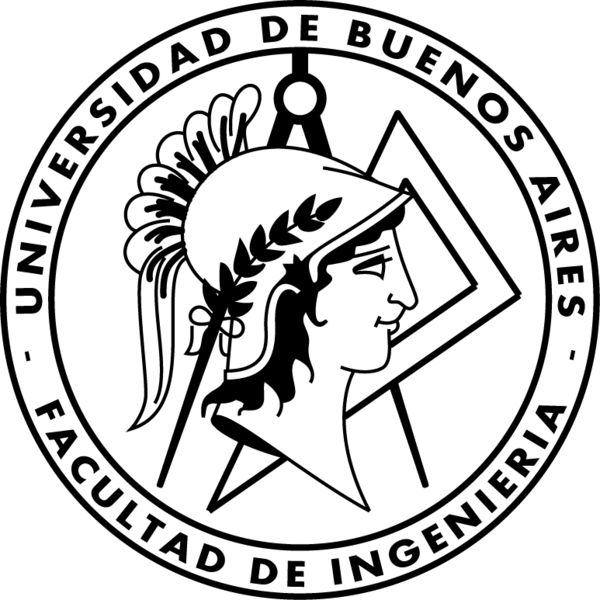
\includegraphics[scale=1]{./img/logo-facu}
\end{figure}

\title{\large\textsc{66.20 - Organización de Computadores}\\
\large Trabajo Práctico Final\\
Predición de Saltos en el camino de datos MIPS 32}

\author{
Andrew Parlane \\
}

\maketitle

\newpage

\tableofcontents

\listoffigures

\newpage

\section{Objetivo}

El objetivo de este trabajo es, usando el program DrMIPS, diseñar, implementar y caracterizar varios predictores de saltos. DrMIPS es un program de fuente abierto escrito en Java, que permite simular el camino de datos de un CPU MIPS. El camino de datos y el conjunto de instrucciones son implementado mediante archivos JSON.

\section{Introducción}

En un CPU monociclo cada instrucción es ejecutado completamente antes de la siguiente comienza. En el caso de un salto condicional esto significa que, es conocido si el salto estará tomado o no, antes de cuando es necesario leer la siguiente instrucción. Mientras que en un CPU con un pipeline, dos o más instrucciones pueden estar ejecutando al mismo tiempo. Así puede ser necesario comenzar leer la siguiente instrucción antes de cuando es conocido si un salto estará tomado o no. Esto es un riesgo de control.

En un CPU MIPS 32 básico el pipeline tiene cinco etapas:

\begin{itemize}
\item IF - Lea la instrucción desde la memoria de instrucciones.
\item ID - Descodifica la instrucción y lea los registros.
\item EX - Ejecuta operaciones ALU.
\item MEM - Escritora / Lectura de la memoria de datos.
\item WB - Escribe el resultado al registro.
\end{itemize}

Por un salto condicional el CPU solo sabe si debería tomar le o no después de la operación ALU. Normalmente resuelve esto en la etapa MEM, así hay tres ciclos donde el CPU no sabe cual instrucciones leer.

Una solución de esto es introducir un "stall" en el pipeline por cada ciclo hasta el resultado de un salto es conocido. Por ejemplo:

\begin{figure}[!htb]
\centering
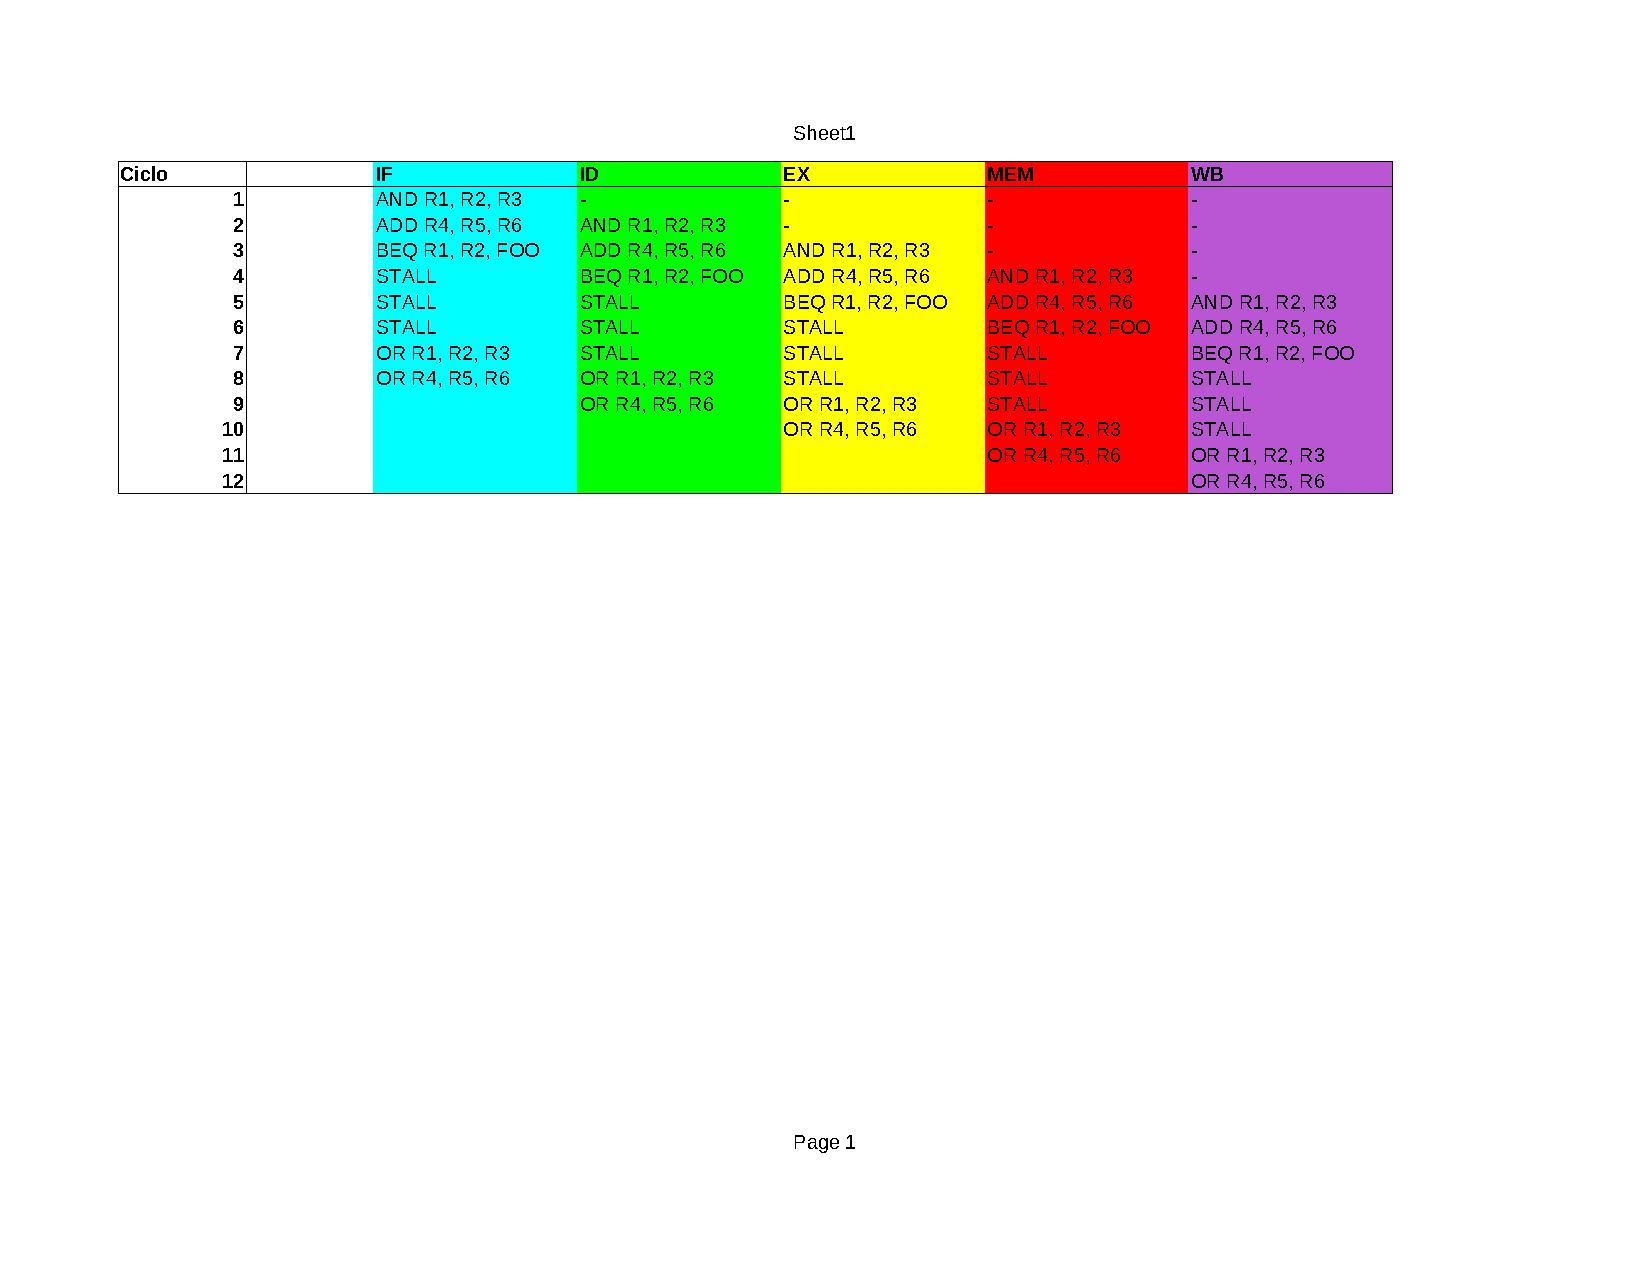
\includegraphics[scale=0.4]{./img/always_stall}
\caption{Evitar riesgos de control mediante stalls.}
\label{fig:always_stall}
\end{figure}

El problema con este método es que no es muy eficiente. Cada salto condicional toma cuatro ciclos para ejecutar. Un mejor método sería intentar predecir si el salto será tomado o no, y si se equivoca, vaciar las primeras tres etapas del pipeline. En este caso el truco es diseñar un predictor muy preciso sin usando demasiado recursos.

También hay otras métodos para mejor el desempeño como "branch delay slots" o resolviendo el salto en una etapa anterior, pero esos son afuera del tema de este proyecto.

\section{Predictores de saltos}
\subsection{Predictores estáticos}

Un predictor de saltos estático elige el mismo acción por cada salto. Hay dos posibilidades: siempre no tomado, siempre tomado.

En el caso de siempre no tomado el procesador sigue leyendo las siguientes instrucciones (PC + 4). En la etapa de MEM si el salto no está tomado, no tiene que hacer nada, la ejecución sigue como normal, pero si el salto está tomado, tiene que vaciar las primeras etapas del pipeline (IF, ID, EX) y ajustar el PC a la dirección nueva. Figura \ref{fig:assume_not_taken_wrong} muestra que pasa cuando un salto es tomado.

\begin{figure}[!htb]
\centering
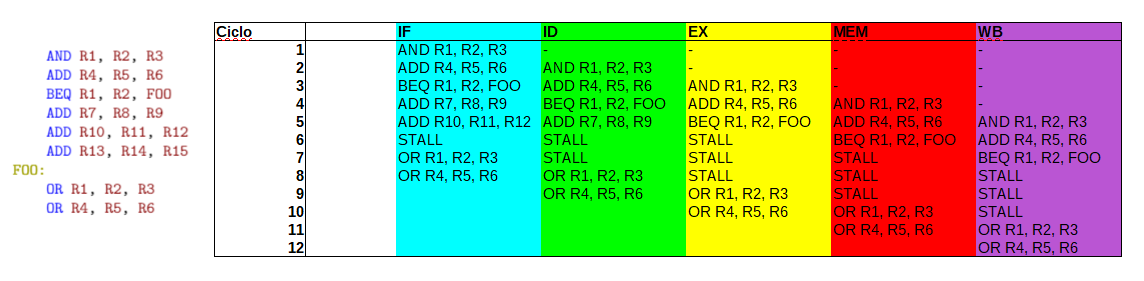
\includegraphics[scale=0.4]{./img/assume_not_taken_wrong}
\caption{Vaciando el pipeline después de una predicción equivocado de salto no tomado.}
\label{fig:assume_not_taken_wrong}
\end{figure}

La otra opción es siempre suponer que el salto será tomado. El problema con este método es que no sabe que es un salto hasta la segunda etapa ID, así siempre tiene que vaciar la primera etapa IF. Si el salto actualmente es tomado, no hay nada más hacer, pero en el caso que no es tomado, tiene que vaciar las primeras tres etapas de nuevo. Figura \ref{fig:assume_taken} muestra los dos casos.

\begin{figure}[!htb]
\centering
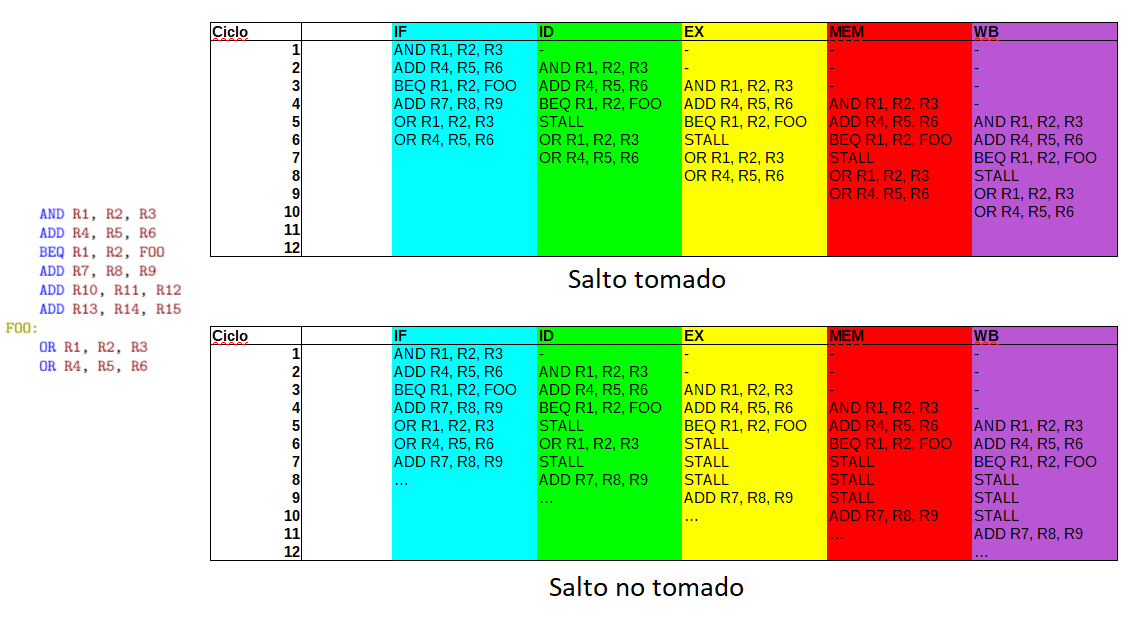
\includegraphics[scale=0.4]{./img/assume_taken}
\caption{El flujo de ejecución con un predictor de saltos siempre tomados.}
\label{fig:assume_taken}
\end{figure}

\subsection{Predictores dinámicos}

Predictores de saltos dinámicos intentan predecir si el salto será tomado o no basado en la historia del salto (historia local) o de todos los saltos (historia global).

\subsubsection{Predictor de historia local}

Un predictor de saltos de historia local usa $2^N$ contadores que saturan, de M bits cada uno. En la etapa ID un contador es direccionado con N bits del PC. Si el valor corriente del contador tiene el bit más significativo encendido predice que el salto estará tomado. En la etapa MEM el contador es actualizado, si el salto actualmente está tomado, se incrementa por uno, y si no, se decrementa por uno. También en la etapa MEM si la predicción estuvo equivocado, vacía las primeras tres etapas del pipeline y ajusta el PC hasta el valor correcto. Figura \ref{fig:local_history} muestra un predictor de historia local.

\begin{figure}[!htb]
\centering
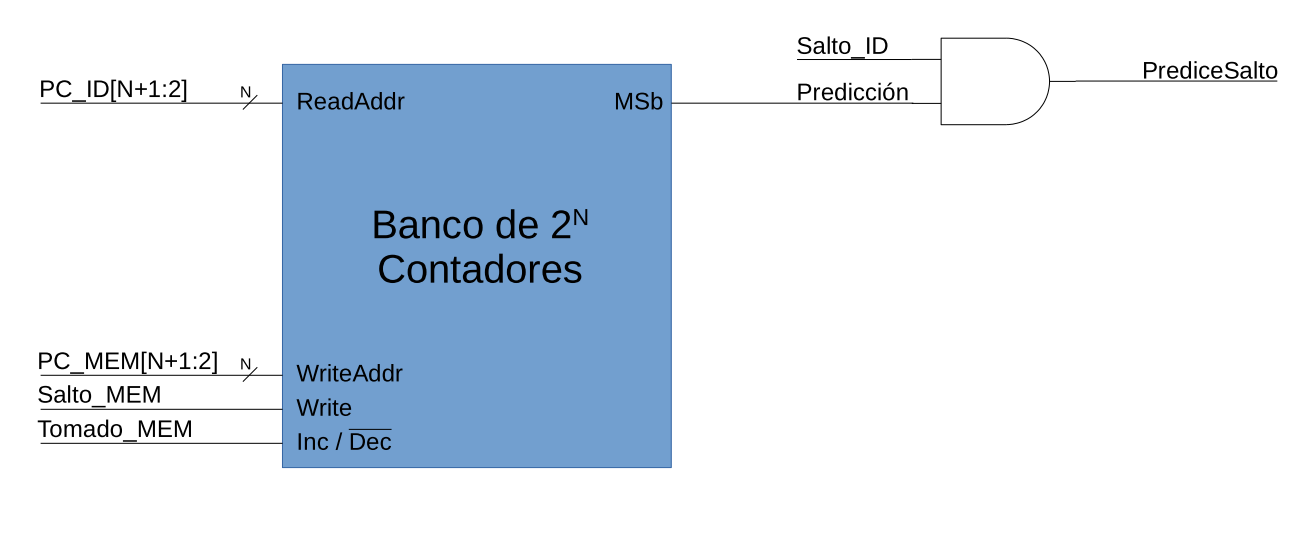
\includegraphics[scale=0.4]{./img/local_history}
\caption{Un predictor de historia local.}
\label{fig:local_history}
\end{figure}

La idea de esto es que si un salto es tomado más frecuentemente que no, el valor del contador normalmente estará cerca el máximo y predice tomado, y viceversa.

Porque hay $2^N$ contadores usamos N bits del PC para direccionar los contadores. En MIPS32 cada instrucción es cuatro bytes, así los dos bits más bajos del PC siempre son ceros. Normalmente usan los siguiente N bits menos significativos. Interferencia ocurre cuando dos saltos direcciona el mismo contador. Eligiendo N es un intercambio entre menos interferencia y la cantidad de memoria necesario para guardar los contadores.

Cada contador tiene M bits, si M es uno el contador solo puede ser 0 o 1, así cada vez predice el mismo de que hizo el salto la última vez. El problema con esto es que no hay histéresis. El siguiente código demuestra esto.

\begin{minted}{C}

while (1)
{
    for (int i = 0; i < 3; i++)
    {
        ...
    }
}

\end{minted}

\begin{tabular}{| r | r r r | r r r |}
\cline{2-7}
\multicolumn{1}{c|}{} & \multicolumn{3}{c|}{M=1} & \multicolumn{3}{c|}{M=2} \\ \hline
i & contador & predicción & Hit / Miss & contador & predicción & Hit / Miss \\ \hline
\multicolumn{7}{|c|}{Primer lazo} \\ \hline
1 &     0 & N & Miss &      0 & N & Miss \\
2 &     1 & T & Hit &       1 & N & Miss \\
3 &     1 & T & Miss &      2 & T & Miss \\

\hline
\multicolumn{7}{|c|}{Segundo lazo} \\ \hline
1 &     0 & N & Miss &      1 & N & Miss \\
2 &     1 & T & Hit &       2 & T & Hit  \\
3 &     1 & T & Miss &      3 & T & Miss \\

\hline
\multicolumn{7}{|c|}{Tercero lazo} \\ \hline
1 &     0 & N & Miss &      2 & T & Hit \\
2 &     1 & T & Hit &       3 & T & Hit  \\
3 &     1 & T & Miss &      3 & T & Miss \\

\hline
\multicolumn{7}{|c|}{Todos los demás} \\ \hline
1 &     0 & N & Miss &      2 & T & Hit \\
2 &     1 & T & Hit &       3 & T & Hit  \\
3 &     1 & T & Miss &      3 & T & Miss \\

\hline
\end{tabular} \\

Si ejecuta este lazo suficiente vecez que los primeras dos iteraciones están despreciable, la tasa del hit para M = 1 es 33\%, y para M = 2 es 66\%. Sin embargo, si M es demasiado grande dura mucho tiempo para llegar al estado de equilibrio.

\subsubsection{Predictor de historia global}

Si dos saltos están correlacionados el resultado de uno puede ser adivinado desde el resultado del otro. Por ejemplo, en el código siguiente, si los dos primeros saltos no están tomados (a == 0 y b == 0) entonces el tercer salto no estará tomado tan poco, siempre que a ni b están modificados adentro de los bloques.

\begin{minted}{C}
    if (a == 0)
    {
        ...
    }
    if (b == 0)
    {
        ...
    }
    if (a == b)
    {
        ...
    }
\end{minted}

Para implementar un predictor de historia global, se usa un registro de desplazamiento de N bits para direccionar $2^N$ contadores que saturan, de M bits cada uno. El resultado actual de cada salto entra el registro, guardando una historia global de los saltos. Figura \ref{fig:global_history} muestra un predictor de historia global.

\begin{figure}[!htb]
\centering
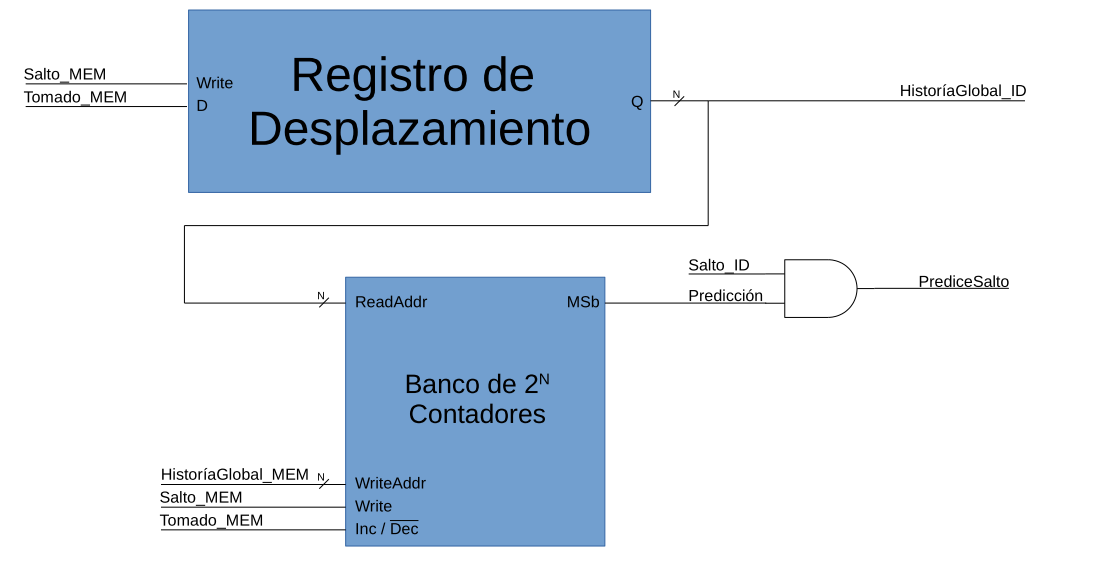
\includegraphics[scale=0.4]{./img/global_history}
\caption{Un predictor de historia global.}
\label{fig:global_history}
\end{figure}

\subsubsection{Predictor de dos niveles}

Un predictor de dos niveles usa ambos de las técnicas anteriores. Un registro de desplazamiento de P bits direcciona $2^P$ bancos de $2^N$ contadores. El contador es direccionado en el banco elegido por N bits del PC. Cada contador tiene M bits. Figura \ref{fig:two_level_predictor} muestra un predictor de dos niveles.

\begin{figure}[!htb]
\centering
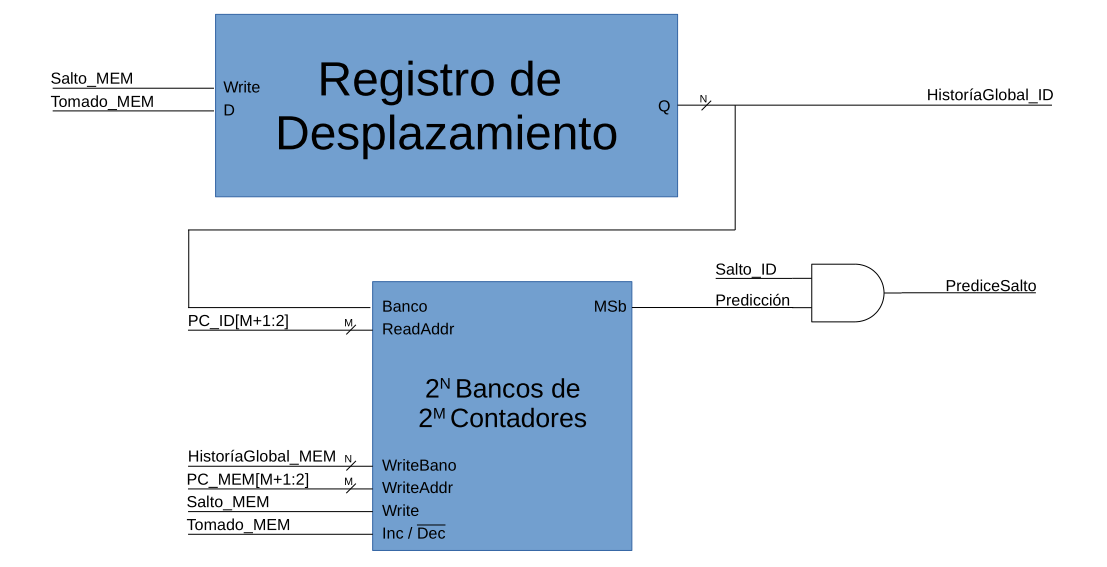
\includegraphics[scale=0.4]{./img/two_level_predictor}
\caption{Un predictor de dos niveles.}
\label{fig:two_level_predictor}
\end{figure}

\subsection{CPI de los predictores}

CPI (Ciclos por instrucción) es una medida de desempeño. Comparando los CPIs por los varios predictores da un idea de que predictor será mejor. Sin embargo no es definitivo, si un predictor tiene un CPI más bajo que otro, pero la implementación significa que la frecuencia del reloj tiene que ser más lento, entonces puede ser menos eficiente.

\begin{tabular}{| l | r  r | r r | }
\cline{2-5}
\multicolumn{1}{c|}{} & \multicolumn{4}{c|}{CPI} \\
\cline{2-5}
\multicolumn{1}{c|}{} & \multicolumn{2}{c|}{Predice Tomado} & \multicolumn{2}{c|}{Predice No Tomado} \\ \hline
Predictor & Tomado & No Tomado & Tomado & No Tomado \\ \hline
Siempre Stall       &   4   &   4   &   4   &   4   \\
Supone No Tomado    &   -   &   -   &   4   &   1   \\
Supone Tomado       &   2   &   4   &   -   &   -   \\
Dinámicos           &   2   &   4   &   4   &   1   \\

\hline
\end{tabular}

El CPI Promedio ($\bar{CPI}$) depende del Hit Rate y del ratio de tomado a no tomado en el programa. Pero es claro que equivocando es muy caro, así el diseño del predictor es muy importante.

\section{Implementación en DrMIPS}

\subsection{Componentes JAVA}

Tuve que implementar unos componentes en JAVA para uso en mis caminos de datos:

\begin{itemize}
    \item Banco de Contadores que Saturan, con el ancho de los contadores y el número de contadores configurable.
    \item Registro de desplazamiento, con el ancho configurable.
    \item Demultiplexador de tamaño configurable.
\end{itemize}

No estoy muy familiar con JAVA pero pude implementar estos componentes sin dificultades, usando el componente del Register File como plantilla, para los primeros dos, y el multiplexador para el último.

DrMIPS tiene bancos de pruebas para cada componente los que están ejecutados como parte del proceso de compilación. He escrito un banco de prueba para cada uno de mis componentes.

\subsection{Camino de Datos}

Empecé con el camino de datas "Pipeline Extended" lo que viene con DrMIPS. Este camino de datos supone que saltos no estarán tomados. Usando eso como base implementé los siguientes diseños:

\begin{itemize}
    \item Siempre Stall.
    \item Supone tomado.
    \item Historia local.
    \item Historia global.
    \item Dos niveles.
\end{itemize}

En los casos de los predictores dinámicos inicializo todos los contadores hasta $2^(M-1) - 1$, así están en el medio del rango en el lado de predecir no tomado.

\subsubsection{Siempre Stall}

En este camino de datos, cuando un Salto es detectado en la etapa de ID, EX, las etapas anteriores están vaciado. En la etapa MEM, si hay un salto y está tomado, vaciamos las etapas anteriores y actualizamos el PC. Figura \ref{fig:always_stall_drmips} muestra el diseño final.

\begin{figure}[!htb]
\centering
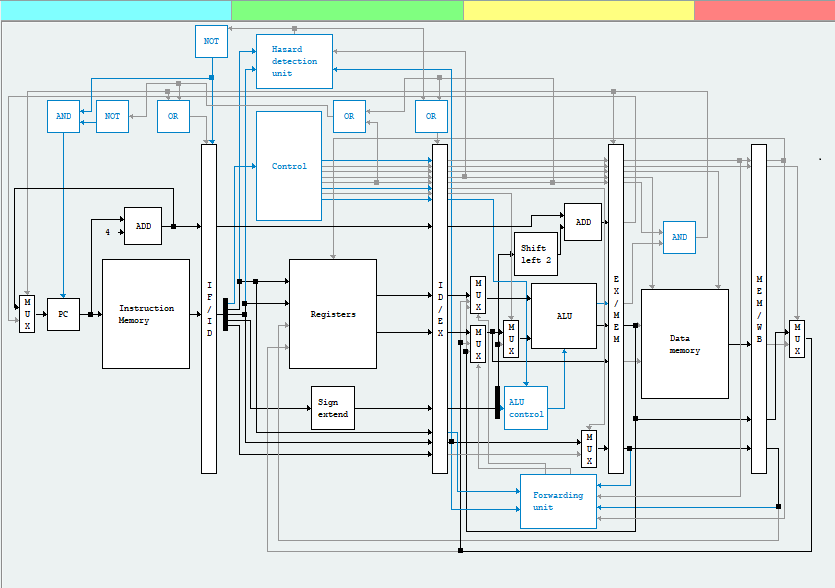
\includegraphics[scale=0.4]{./img/always_stall_drmips}
\caption{El camino de datos que siempre stalls.}
\label{fig:always_stall_drmips}
\end{figure}

\subsubsection{Supone tomado}

En este camino de datos, tuve que mover la calculación del target a la etapa ID desde la etapa EX. Añadí un extra mux para elegir como actualizar el PC (PC+2, target en ID, target correcto en MEM). Vacío IF cuando hay un salto en ID Y finalmente en vez de vaciando las etapas anteriores en MEM cuando el salto actualmente es tomado, hago cuando el salto no es tomado. Figura \ref{fig:predict_taken_drmips} muestra el diseño final.

\begin{figure}[!htb]
\centering
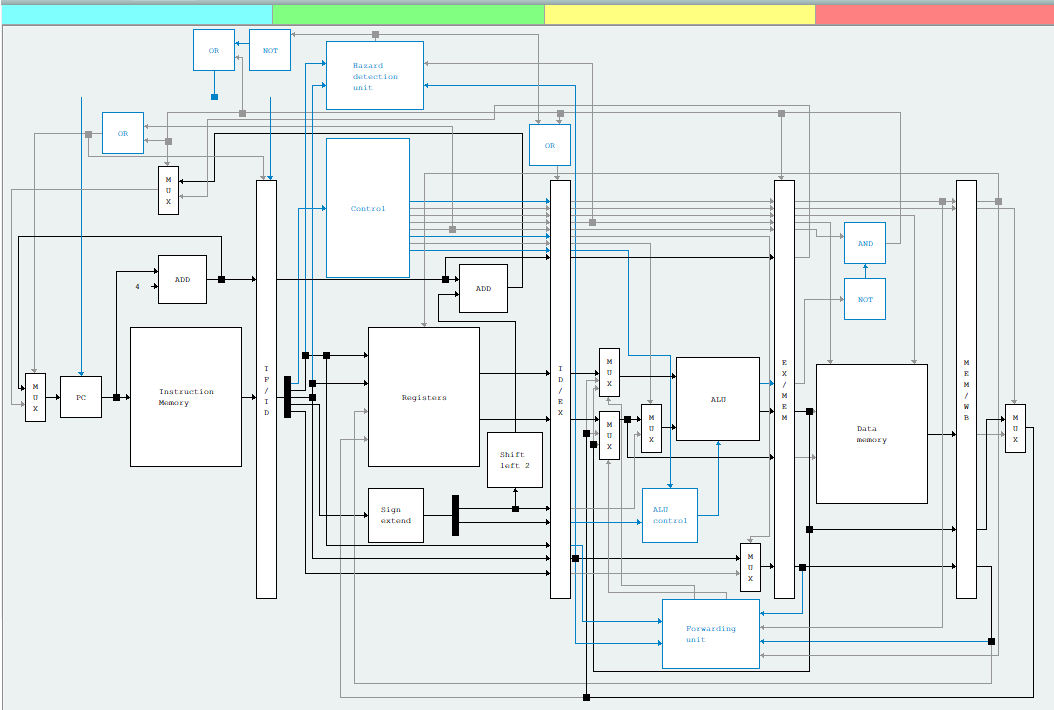
\includegraphics[scale=0.4]{./img/predict_taken_drmips}
\caption{El camino de datos con un predictor estático supone tomado.}
\label{fig:predict_taken_drmips}
\end{figure}

\subsubsection{Historia Local}

En este camino de datos uso mi banco de contadores para predecir el salto en la etapa ID, y actualizarle en la etapa MEM. Como siemper hay lógica para vaciar las etapas IF, ID y EX cuando es necesario, el único diferencia es que solo vacia IF desde ID si predice un salto. Figura \ref{fig:local_history_drmips} muestra el diseño final.

\begin{figure}[!htb]
\centering
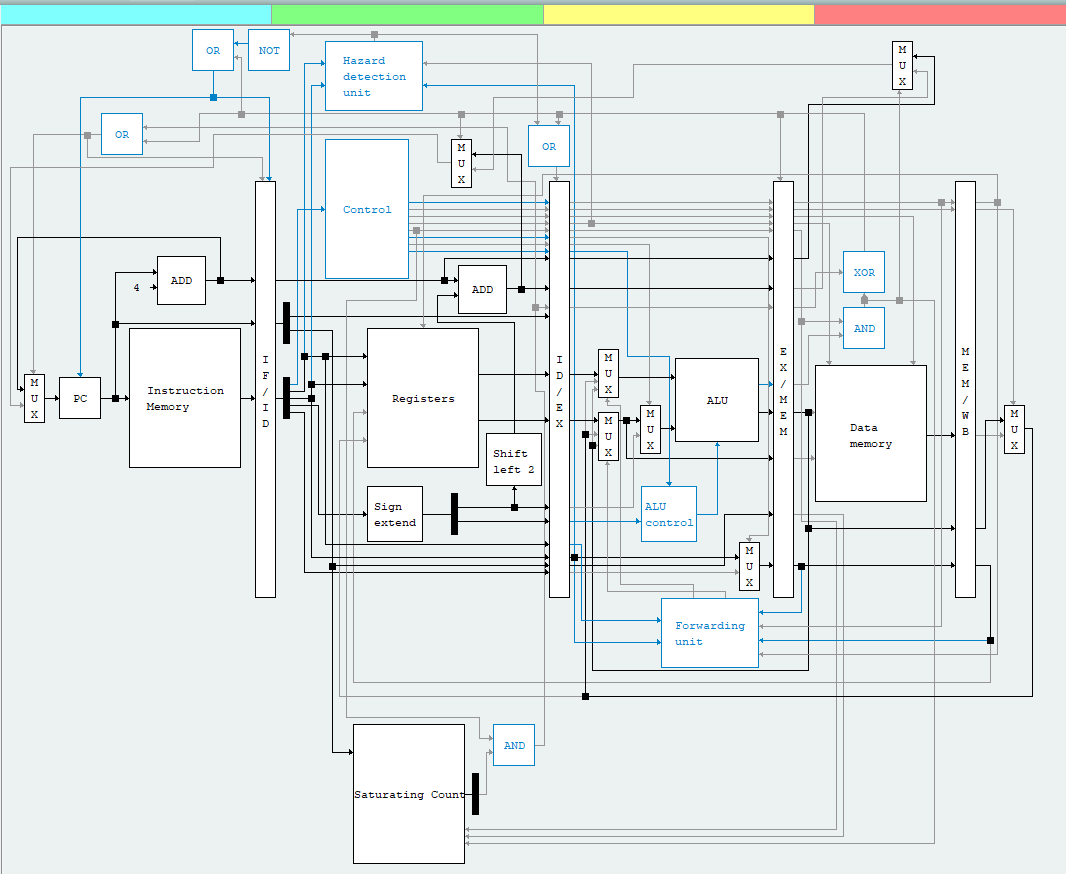
\includegraphics[scale=0.4]{./img/local_history_drmips}
\caption{El camino de datos con un predictor de historia local.}
\label{fig:local_history_drmips}
\end{figure}

\subsubsection{Historia Global}

En este camino de datos uso mi registro de desplazamiento para direccionar el banco de contadores. En la etapa MEM actualizo el registro de desplazamiento tanto como el contador usado para la predicción. Figura \ref{fig:global_history_drmips} muestra el diseño final.

\begin{figure}[!htb]
\centering
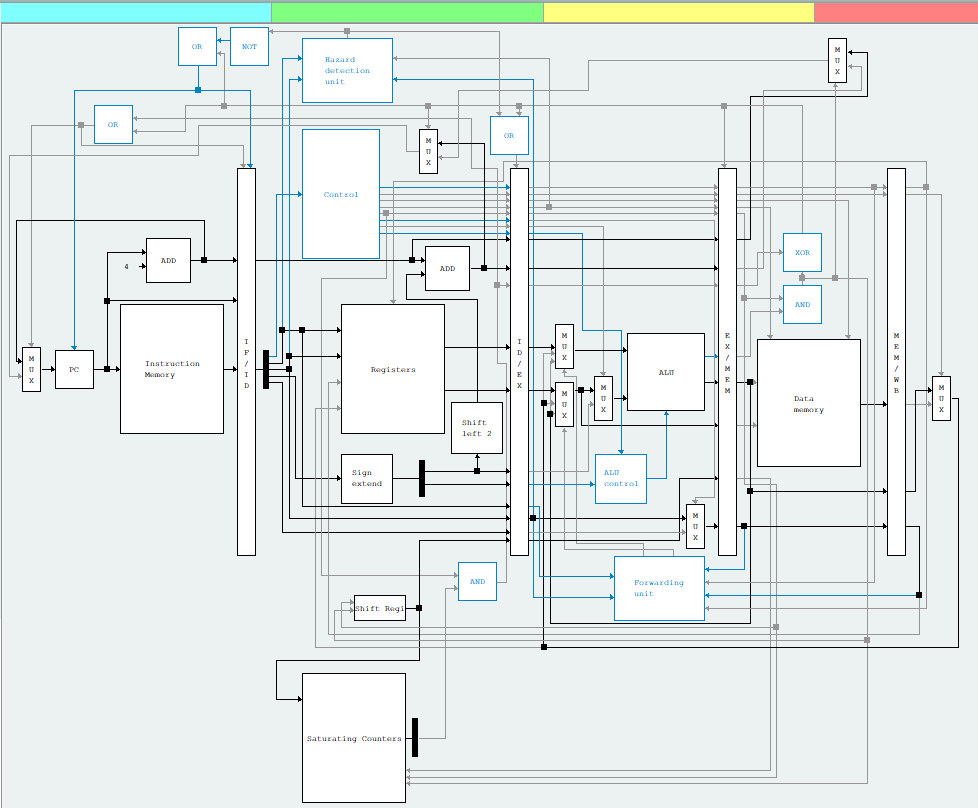
\includegraphics[scale=0.4]{./img/global_history_drmips}
\caption{El camino de datos con un predictor de historia global.}
\label{fig:global_history_drmips}
\end{figure}

\subsubsection{Dos Niveles}

Finalmente hay el predictor de dos niveles. Funciona parecido al predictor de historia local, pero en vez de tener un banco de contadores hay cuatro direccionado con la historia global. El única otra cosa interesante es el uso de mi demultiplexor para elegir cual banco actualizar en la etapa MEM. Figura \ref{fig:two_level_drmips} muestra el diseño final.

En el camino de datos de historia local y historia global no es tan difícil cambiar el número de contadores sus anchos y el ancho del registro de desplazamiento. Pero en este camino de datos es mucho más difícil cambiar el número de banco de contadores. Si querrías aumentar el ancho del registro de desplazamiento un bit, tienes que manualmente añadir y conectar cuatro más bancos de contadores mediante la manipulación de archivos JSON, que es muy laborioso. Una optimización futuro será añadir un nuveo componente JAVA que tiene un conjunto de bancos de contadores, como lo que es mostrado en Figura \ref{fig:two_level_predictor}.

\begin{figure}[!htb]
\centering
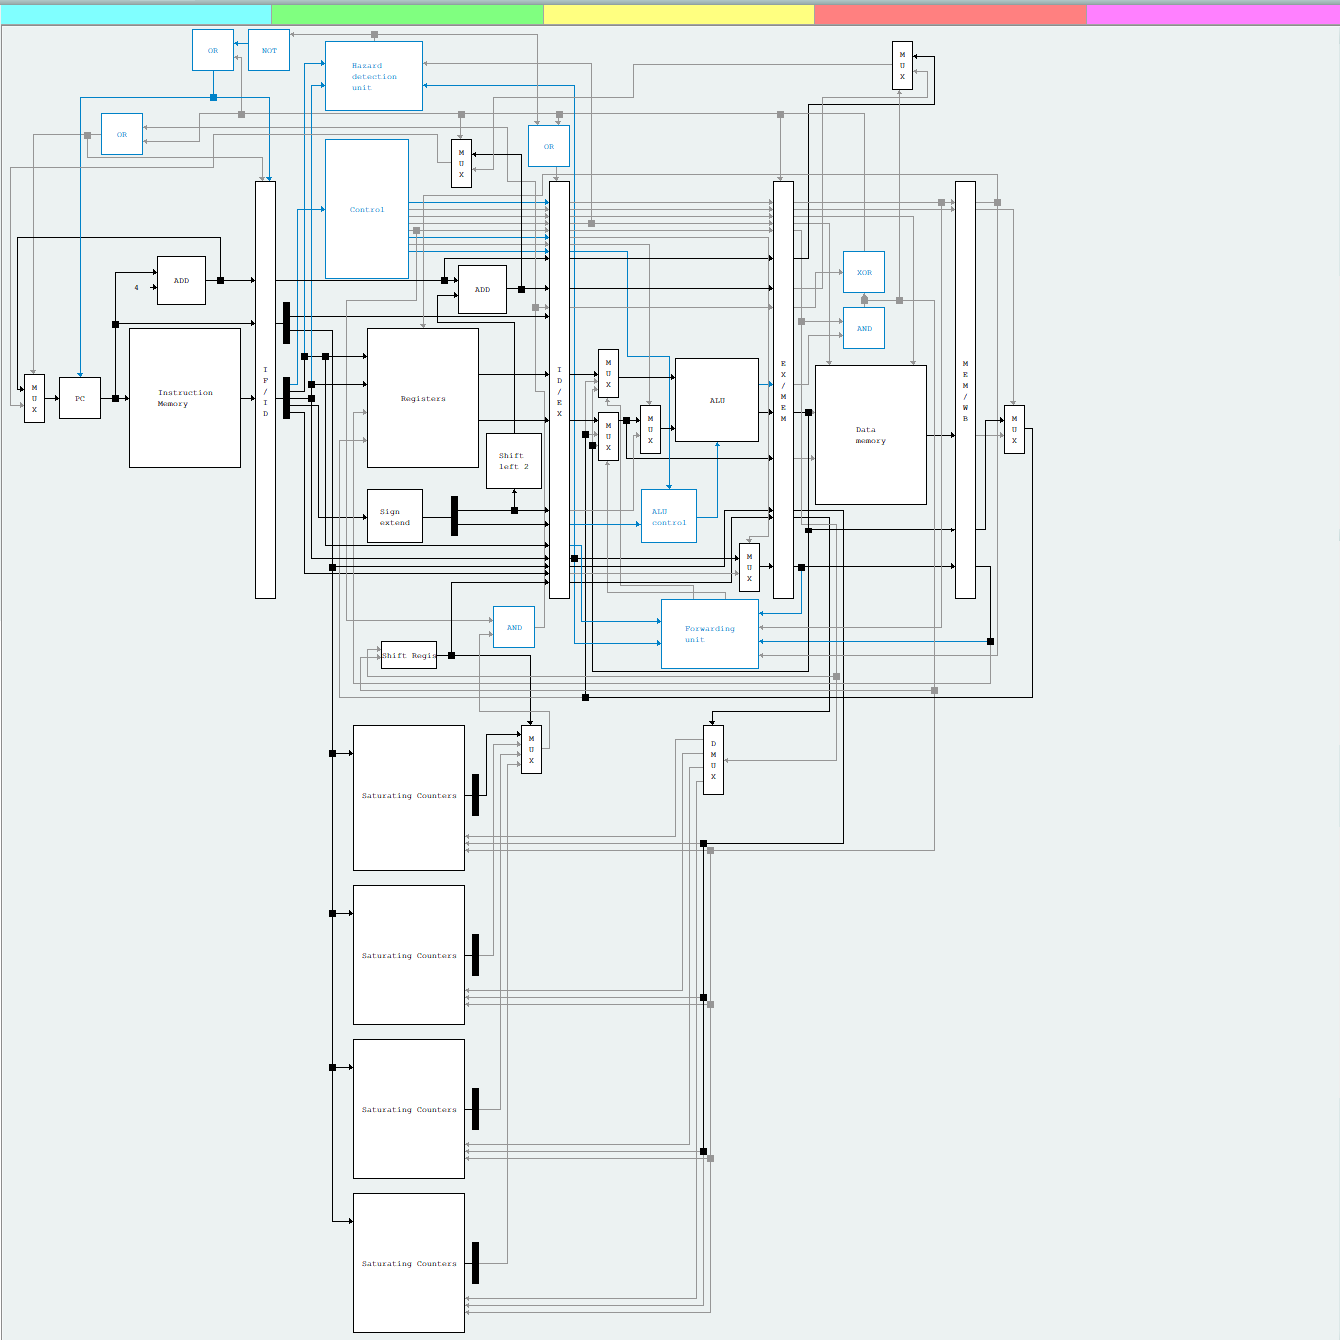
\includegraphics[scale=0.4]{./img/two_level_drmips}
\caption{El camino de datos con un predictor de dos niveels.}
\label{fig:two_level_drmips}
\end{figure}

\subsection{Depurando}

Durante la implementación del algoritmo quicksort para analizar el desempeño de los predictores, encontré un bug donde mi algoritmo no estuvo ordenando los valores correctamente. Mientras estuve depurando esto, encontré que el comportamiento estuvo diferente entre los caminos de datos "Pipeline Extended" y "Unicyle Extended". El bug estuvo en el diseño del camino de datos "Pipeline Extended" y no en mi algoritmo.

Para encontrar este problema tuve que ir paso por paso por miles de ciclos. A final implementé breakpoints en DrMIPS, así que pude ejecutar mi algoritmo hasta una dirección para acelerar depurando.

El bug estuvo que cuando la Hazzord Detection Unit encuentra un hazzard desactiva escritos al PC. Si en el mismo cíclo la etapa MEM está actualizando el PC debido a un salto tomado, el escrito es ignorado y el flujo sigue por el salto equivocado. Arreglé este bug en dos de los pipelines y generé un push request al upsteam despositivo. Después tuve que arreglar el bug en mis pipelines también.

\subsection{Scripts}

Solo realicé una implementación de cada camino de datos, pero quise una forma analizarles con un rango del número de contadores $(2^N)$ y sus anchos M. Para hacer esto, escribí unos scripts en python para modificar los archivos JSON.

También escribí otro script en python para graficar los "Hit Rates" de los predictores por todos los parámetros.

\section{Algoritmos de prueba}

Cuando llegó a la hora de escribir código para analizar el desempeño de cada camino de datos, encontré unas limitaciones de DrMIPS:

\begin{itemize}
    \item Por defecto solo ejecuta mil ciclos, después tienes que hace clic ejecuta de nuevo. Incrementé este limite a diez mil, que es mejor pero no es ideal.
    \item Si ejecutas más de 80.000 ciclos DrMIPS falla por falta de memoria.
    \item Las instrucciones implementado por defectos están limitados. La falta de JR es espacialmente molesto porque no puedes devolver desde una función, ni usa algoritmos recursivos. Podría haber implementado la instrucción JR pero habría sido necesario implementarle por cada camino de datos, y aun haciéndolo una vez es bastante laborioso.
    \item La memoria de datos es de solo 400 bytes.
\end{itemize}

Por estos razones estuve limitado en los algoritmos que pude implementar.

Nota que decidí no seguir un ABI en mi código, uso cualquier registros y no tengo un stack (excepto de en la prueba de quicksort).

\subsection{Lazo}

\begin{minted}{ASM}
li $t0, 0
li $t1, 99
start:
	addi $t0, $t0, 1
	ble $t0, $t1, start
\end{minted}

Este algoritmo muestra como los predictores diferentes funcionan con un salto que casi siempre es tomado.

\subsection{Mayor Denominador Común}

En esta prueba calculo el mayor denominador común por todos (GCD) los pares de números en el rango de 50-59 y 90-99.

\begin{minted}{ASM}
    li $s2, 99                      # maxA = 99;
    li $s3, 59                      # maxB = 59;
    li $s4, 0                       # idx = 0;

    li $s0, 90                      # a = 90;
a_loop_start:                       # do {
    li $s1, 50                      #   b = 50;
b_loop_start:                       #   do {
    move $t0, $s0                   #
    move $t1, $s1
    b gcd_loop_start                #     res = gcd(a,b);
gcd_return:
    sw $t2, 0($s4)                  #     results[idx] = res;
    addi $s4, $s4, 4                #     idx++;
    addi $s1, $s1, 1                #     b++
    ble $s1, $s3, b_loop_start      #   } while (b <= maxB)
    addi $s0, $s0, 1                #   a++
    ble $s0, $s2, a_loop_start      # } while (a <= maxA)
    b endProg                       # return;

gcd_loop_start:                     # while (1) {
    beq $t0, $zero, ret_b           #   if (a == 0) return b;
    beq $t1, $zero, ret_a           #   if (b == 0) return a;
    beq $t0, $t1, ret_a             #   if (a == b) return a;
    bge $t0, $t1, a_greater_than_b  #   if (a < b) {
    sub $t1, $t1, $t0               #     b -= a;
    b gcd_loop_start                #   }
a_greater_than_b:                   #   else {
    sub $t0, $t0, $t1               #     a -= b;
    b gcd_loop_start                #   }
                                    # }

ret_a:
    move $t2, $t0
    b gcd_return
ret_b:
    move $t2, $t1
    b gcd_return

endProg:
\end{minted}

\subsection{Bubble Sort}

\begin{minted}{ASM}

# Cargar data generado por un generador de números random.
# Uso 50 valores entre 0 y 100.
li $t0, 94
li $t1, 0
sw $t0, 0($t1)
li $t0, 29
addi $t1, $t1, 4
sw $t0, 0($t1)
li $t0, 87
addi $t1, $t1, 4
sw $t0, 0($t1)
...

# t1 dirección de el último valor
# t2 cambiado? flag
# t3 dirección de valor corriente
# t4 valor1
# t5 valor2
startOuter:                         # do
                                    # {
    li $t2, 0                       #   bool cambiado = 0;
    li $t3, 0                       #   uint8_t *ptr = 0; // primer valor es a dirección 0

startInner:                         #   do
                                    #   {
        lw $t4, 0($t3)              #     valor1 = ptr[0];
        lw $t5, 4($t3)              #     valor2 = ptr[1];
        ble $t4, $t5, noSwap        #     if (valor1 > valor2)
                                    #     {
        sw $t4, 4($t3)              #       ptr[1] = valor1;
        sw $t5, 0($t3)              #       ptr[0] = valor2;
        li $t2, 1                   #       cambiado = 1;
                                    #     }
noSwap:
        addi $t3, $t3, 4            #     ptr++;
        beq $t3, $t1, endLoop
        b startInner                #   } while (ptr != úlimo)

endLoop:
        li $t6, 1
        beq $t2, $t6, startOuter    # } while (cambiado)
\end{minted}

\subsection{Quick Sort}

El algoritmo básico de quicksort es:

\begin{minted}{C}
void quickSort(int *first, int *last)
{
    if (low < high)
    {
        int *j = ...;

        quickSort(first, j - 1);
        quickSort(j + 1, last);
    }
}
\end{minted}

Es una función recursivo, así es necesario tener un stack. El stack frame necesita guardar tres valores:

\begin{itemize}
    \item La dirección a volver (\$RA).
    \item El pivot (j).
    \item La dirección de la última valor (last).
\end{itemize}

Implementé un stack que crece hacia abajo desde el fin de memoria. Porque solo hay 400 bytes de memoria de datos y usa las primeras 200 bytes por la lista de valores, solo hay 200 bytes disponibles por el stack. Mi implementación en C me muestra que la profundidad máxima es 13 llamadas por la misma lista de datos. 13 stack frames de 12 bytes cada uno significa que necesita 156 bytes por el stack, y tiene 200 bytes, así funciona.

Por la falta de la instruucción JR no puedo solo guardar la dirección a volver como normal. Tuve que usar un valor para indicar cual etiqueta usar. Aquí es el código relevante.

\begin{minted}{ASM}
qsort:
    ...

    # guarda los valores en el stack
    subi $sp, $sp, 12
    sw $ra, 8($sp)
    sw $t2, 4($sp)
    sw $a1, 0($sp)

    # queremos volver a retRecursive1
    li $ra, 1
    ...
    b qsort                 #   qsort(first, j-1);
retRecursive1:

    # queremos volver a retRecursive2
    li $ra, 2
    ...
    b qsort                 #   qsort(j+1,last);
retRecursive2:

    # recuperar $ra del stack
    lw $ra, 8($sp)

    # volver al último stack frame.
    addi $sp, $sp, 12

    # return
    beq $ra, $zero, retRecursive1   # if ($ra == 0) return to retRecursive1
    li $s0, 1
    beq $ra, $s0, retRecursive2     # else if ($ra == 1) return to retRecursive2

endProg:                            # else exit()
\end{minted}

\section{Resultados}

\subsection{Predictores Estáticos}

Ejecuté cada prueba para los tres predictores estáticos. Los resultados están:

\begin{tabular}{| l | r |  r r | r r | r r | }
\cline{3-8}
\multicolumn{2}{c|}{} & \multicolumn{2}{c|}{Siempre Stall} & \multicolumn{2}{c|}{Predecir NT} & \multicolumn{2}{c|}{Predecir T} \\ \hline
Prueba &  Saltos & CPI & HR\% & CPI & HT\% & CPI & HR\% \\ \hline
Loop        & 100  & 2.0 & 0.0 & 2.0 & 1.0  & 1.3 & 99.0 \\
GCD         & 6256 & 2.6 & 0.0 & 1.7 & 64.2 & 2.6 & 35.8 \\
Bubble Sort & 6909 & 2.1 & 0.0 & 1.8 & 41.7 & 1.8 & 58.3 \\
Quick Sort  & 1411 & 1.9 & 0.0 & 1.6 & 51.6 & 1.7 & 48.4 \\
\hline
\end{tabular}

Es claro que la efectividad del predictor tiene un impacto grande en el desempeño del programa. En la prueba de bubble sort el predictor T tiene un mejor hit rate, pero el CPI promedio es igual al predictor NT, esto es porque una predicción correcta de T cuesta dos ciclos mientras una predicción correcta de NT cuesta solo un ciclo. En el caso del lazo el predictor T es mucho mejor que el predictor NT, pero en general el predictor NT es mejor.

\subsection{Predictores Dinámicos}

Ejecuté cada prueba con cada predictor por N entre 1 y 6, y M entre 1 y 6.

Todo el data crudo puede estar encontrado en mi github en el archivo data/analysis.ods, aquí solo pongo los pedazos interesantes.

El diseñador de un CPU quiere que su predictor de saltos tiene el mejor desempeño posible por un mínimo de recursos. Los recursos principales son área y potencia, aquí solo trato de área porque potencia es difícil medir y depende mucho del tecnología de fabricación, mientras área es directamente vinculado con el número de bits usados que es una métrica mucho más fácil usar.

Calculé cuantos bits cada predictor usa por cada par N y M:

\begin{itemize}
    \item Historia Local - Hay $2^N$ contadores, cada uno tiene M bits. Así hay $ M * 2^N $ bits total.
    \item Historia Global - Hay $2^N$ contadores, cada uno tiene M bits, y hay un registro de desplazamiento de N bits. Así hay $ M * 2^N + N $ bits total.
    \item Dos Niveles - Hay 4 bancos de $2^N$ contadores, cada uno tiene M bits, y hay un registro de desplazamiento de 2 bits. Así hay $ 4M * 2^N + 2 $ bits total.
\end{itemize}

Después usé python para dibujar unos gráficos mostrando el CPI y HR contra el número de bits usado. Nota que por el predictor de historia local, los pares de parámetros: (n=2, m=4), (n=3, m=2), (n=4, m=1) todos usan 16 bits. Así en los gráficos podríamos tener un número de bits con más de un punto de dato.

Que encontré es hasta un limite hay un fuerte relación entre número de bits y el HR y el CPI, después de ese limite, el HR y el CPI no cambian mucho y a veces empeoran. Figura \ref{fig:predictor_superplot} muestra estos resultados. Por los predictores de historia local y historia global ese limite es acerca 75 bits, pero en el caso del predictor de dos niveles el limite es acerca 200 bits. Esto indique que por mis pruebas el predictor de historia global necesita más bits para estar efectivo.

\begin{figure}[!htb]
\centering
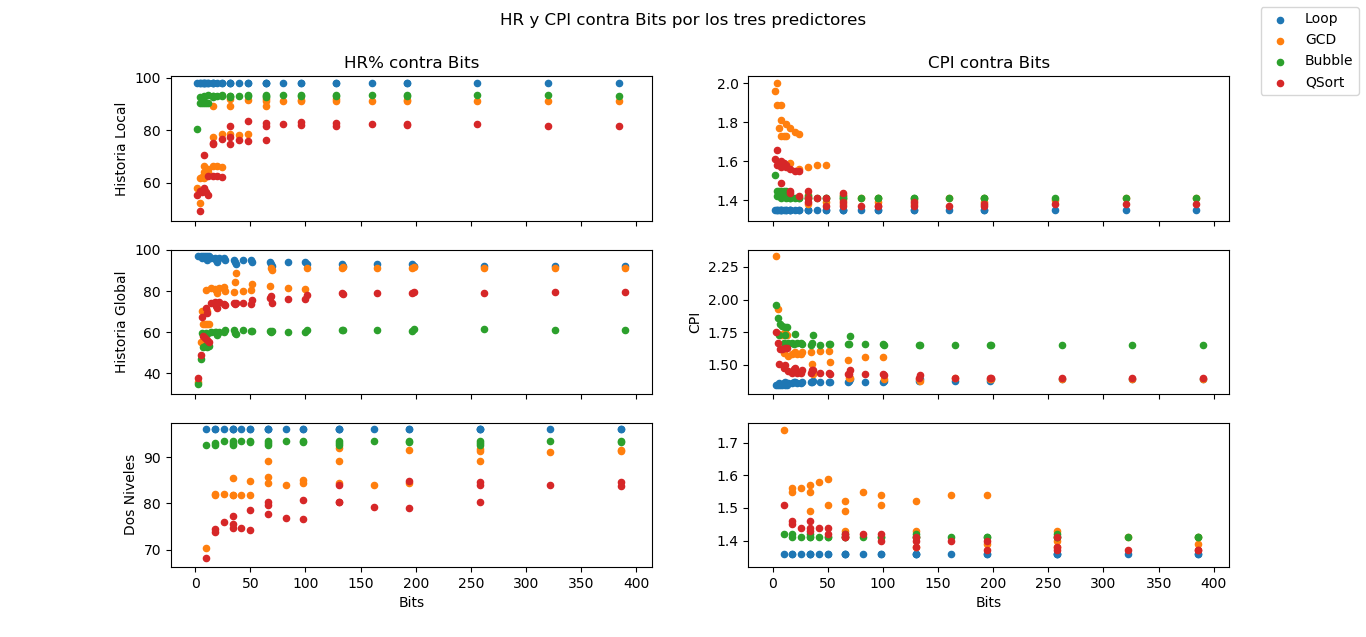
\includegraphics[scale=0.4]{./img/predictor_superplot}
\caption{Gráficos de CPI y HR\% contra bits por cada predictor.}
\label{fig:predictor_superplot}
\end{figure}

Figura \ref{fig:algos_superplot} muestra como se comparan los predictores por cada algoritmo. El predictor de historia global es el peor en todos los casos excepto de por el GCD donde es equivalente del historia local y dos niveles. Los predictores de historia local y de dos niveles estan muuy parecidos pero el de historia local está mejor por menos bits.

\begin{figure}[!htb]
\centering
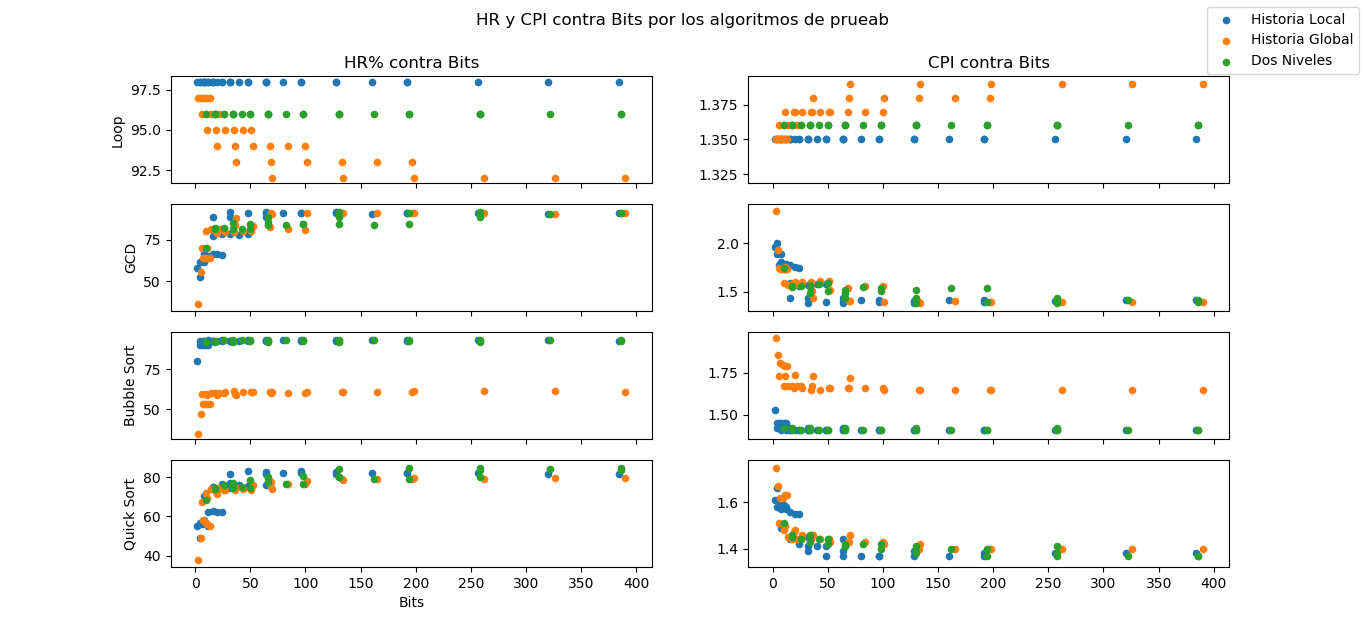
\includegraphics[scale=0.4]{./img/algos_superplot}
\caption{Gráficos de CPI y HR\% contra bits por cada prueba.}
\label{fig:algos_superplot}
\end{figure}

En Figura \ref{fig:algos_superplot} hay un punto de historia local cerca 50 bits que tiene un muy bueno CPI por todos los algoritmos. Volviendo a mi data cruda lo encontré viene de (N=4, M=3). La siguiente tabla muuestra como se compara con el mejor de cada predictor.

\begin{tabular}{|l|rr|rr|rr|rr|}
\cline{2-9}
\multicolumn{1}{c}{} & \multicolumn{2}{|c}{Loop} & \multicolumn{2}{|c}{GCD} & \multicolumn{2}{|c}{Bubble Sort} & \multicolumn{2}{|c|}{Quick Sort} \\ \hline
Predictor & HR\% & CPI & HR\% & CPI & HR\% & CPI & HR\% & CPI \\ \hline
Historia Local Mejor & 98.00	& 1.35 & 91.90 & 1.38 & 93.47 & 1.41 & 83.35 & 1.37 \\
Historia Global	Mejor & 97.00	& 1.35 & 91.62 & 1.38 & 61.63 & 1.65 & 79.52 & 1.40 \\
Dos Niveles Mejor & 96.00	& 1.36 & 91.86 & 1.38 & 93.56 & 1.41 & 84.76 & 1.37 \\ \hline
Historia Local (N=4, M=3) & 98.00	& 1.35 & 91.54 & 1.39 & 93.47 & 1.41 & 83.35 & 1.37 \\
\hline
\end{tabular}

Tiene el mejor CPI en cada caso excepto del GCD y en ese caso es muy cerca.

\section{Conclusión}

Durante este proyecto aprendí los siguientes:

\begin{itemize}
    \item Cómo funciona DrMIPS.
    \item Cómo leer y escribir archivos de JSON mediante JAVA y python y de mano.
    \item Cómo funcionan varios predictores de saltos.
    \item La importancia de benchmarks.
    \item Cómo usar python para analizar data y dibujar gráficas.
\end{itemize}

Si supongamos que mis algoritmos de pruebas están representativos del código que este CPU va a ejecutar en el mundo real, entonces el predictor de saltos más óptimo es lo de la historia local con $2^4 = 16$ contadores de 3 bits cada uno. Creo que esta suposición es valido debidos a las restricciones en las instrucciones disponibles y en el tamaño de memoria de datos.

Los benchmarks son el parte más importante al diseño de un predictor de saltos tanto cómo al CPU entero. Si no están representativos de caso de uso real, el diseño no va a estar óptimo. Habría sido mejor tener más benchmarks incluyendo unos que están más complicados y ejecutan para más tiempo. Creo habría comenzado encontrar que el predictor de saltos de dos niveles estuvo mejor que lo del historia local.

Sugiero que un proyecto por el futuro será mejorar DrMIPS para quitar estos limites en el tamaño de memoria de datos y el número de ciclos máximos, implementar más instrucciones, especialmente JR y implementar benchmarks más complicados.

\section{Código}

Todo el código fuente y datos crudos son disponible en mi repositorio de GitHub:  \href{https://github.com/andrewparlane/fiuba6620_orga_de_compus/tree/master/tpFinal}{Organización de computadores} y \href{https://github.com/andrewparlane/drmips}{DrMIPS}.

\end{document}